There are various functions that facilitate the manipulation of the networks, the copying and pasting of its subparts, the selection of some portions of it, etc. Those of them are missing in Cytoscape.
\subsection{Select Edges between Selected Nodes}
\textbf{Plugins$\Rightarrow$BiNoM 2.0$\Rightarrow$BiNoM Utilities$\Rightarrow$Select Edges between Selected Nodes} or f8\\
When some components are selected by their names (Select$\Rightarrow$Nodes$\Rightarrow$By Name) or simply with the mouse, the edges between the nodes are not selected. This function allows to remedy this problem.\\\\
This might be especially useful when the selection is copied and pasted in another network, although it is possible to paste the nodes with the edges connecting them, without selecting them, by choosing File$\Rightarrow$New$\Rightarrow$Network$\Rightarrow$From selected nodes, all edges when pasting them.

\subsection{Select upstream neighbours}
\textbf{Plugins$\Rightarrow$BiNoM 2.0$\Rightarrow$BiNoM Utilities$\Rightarrow$Select upstream neighbours} or ctrl+8\\
Select upstream neighbours of selected nodes. Whole upstream neighbours can be selected by repeating the command until no more node is selected.

\subsection{Select downstream neighbours}
\textbf{Plugins$\Rightarrow$BiNoM 2.0$\Rightarrow$BiNoM Utilities$\Rightarrow$Select downstream neighbours} or ctrl+9\\
Select downstream neighbours of selected nodes. Ditto downstream.

\subsection{Double Network Differences}
\textbf{Plugins$\Rightarrow$BiNoM 2.0$\Rightarrow$BiNoM Utilities$\Rightarrow$Double Network Differences}\\
A network is composed of nodes and edges. With this command, two networks A and B can be compared and the difference observed between the two is created in two new graphs: A-B for the differences of A compared to B (A-A$\cap$B), and B-A for the differences of B compared to A (B-A$\cap$B). Note that in the output networks, the layout of the first graph is conserved.

\subsection{Update Networks}
\textbf{Plugins$\Rightarrow$BiNoM 2.0$\Rightarrow$BiNoM Utilities$\Rightarrow$Update Networks}\\
When a network is modified, it is possible to update all the networks that are related to it, either because they are modules, sub-networks or older versions of it. That way, any changes, additions or deletions in a network can be propagated to the sub-parts that are derived from the initial version of that network. The user specifies which network is added, which one is deleted (when necessary) and which networks need to be updated in the proposed list.\\\\
Whatever is added or deleted in each sub-network is presented to the user in a separate window before any action is made. The user can agree or disagree by checking or unchecking the box in front of the network names. The previous version of the updated diagrams will not be deleted but saved under \textit{network\_name.xml\_old}. 

\subsection{Update connections from other network}
\textbf{Plugins$\Rightarrow$BiNoM 2.0$\Rightarrow$BiNoM Utilities$\Rightarrow$Update connections from other network}\\
The dialog (figure~\ref{Update_connections}) propose to select:
\begin{itemize}
\item From network, the reference network where are the connections.
\item Networks to update: networks in which connections are copied.
\end{itemize}
\begin{figure}[h]
\centering
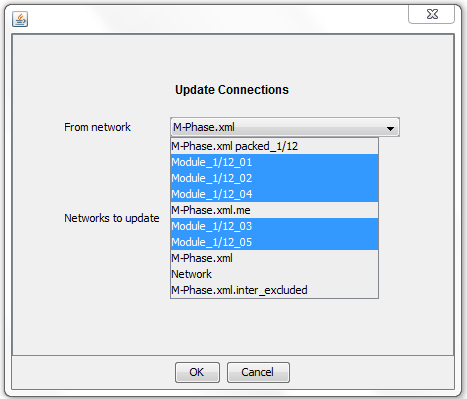
\includegraphics{graphics/Update_connections}
\caption{Update connections from other networks Dialog}
\label{Update_connections}
\end{figure}
Some connections may be duplicated. So a Cytoscape command (version 8.0) may be used to delete them:\\
\textbf{Plugins$\Rightarrow$Network Modifications$\Rightarrow$Remove Duplicated Edges}

\subsection{Merge Networks and Filter by Frequency}
\textbf{Plugins$\Rightarrow$BiNoM 2.0$\Rightarrow$BiNoM Utilities$\Rightarrow$Merge Networks and Filter by Frequency}\\
Create a network by merging the selected networks where the percentage of common nodes is geater then intersection threshold (see dialog figure~\ref{Merge_Networks_and_Filter}) .\\\\
\begin{figure}[h]
\centering
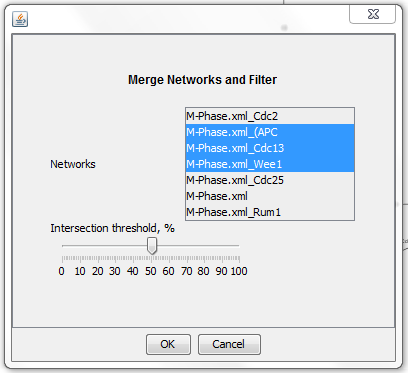
\includegraphics{graphics/Merge_Networks_and_Filter}
\caption{Merge Networks and Filter by Frequency Dialog}
\label{Merge_Networks_and_Filter}
\end{figure}

\subsection{Clipboard}
The description of the commands, which work only inside a Cytoscape session, is self-explanatory.\\
\textbf{Plugins$\Rightarrow$BiNoM 2.0$\Rightarrow$BiNoM Utilities$\Rightarrow$Clipboard$\Rightarrow$Copy selected nodes and edges to clipboard}\\
\textbf{Plugins$\Rightarrow$BiNoM 2.0$\Rightarrow$BiNoM Utilities$\Rightarrow$Clipboard$\Rightarrow$Add selected nodes and edges to clipboard}\\
\textbf{Plugins$\Rightarrow$BiNoM 2.0$\Rightarrow$BiNoM Utilities$\Rightarrow$Clipboard$\Rightarrow$Paste nodes and edges from clipboard}\\
\textbf{Plugins$\Rightarrow$BiNoM 2.0$\Rightarrow$BiNoM Utilities$\Rightarrow$Clipboard$\Rightarrow$Show clipboard contents}\\